\documentclass[11pt]{article}
%\usepackage{fullpage,graphicx,algorithm,algorithmic,bm,amsmath,amsthm,amssymb,color,hyperref,cite,natbib}

% if you need to pass options to natbib, use, e.g.:
%\PassOptionsToPackage{numbers}{natbib}
\usepackage{natbib,fullpage}
\usepackage{bm,amsmath,amsthm,amssymb,multicol,algorithmic,algorithm,enumitem}
\usepackage{wrapfig,lipsum}
\usepackage[textwidth=1cm,textsize=footnotesize]{todonotes}

% ready for submission
\usepackage{neurips_2020}

\usepackage[colorlinks=true,
linkcolor=red,
urlcolor=blue,
citecolor=blue]{hyperref}
\usepackage{hyperref}
\usepackage{cleveref}

\setlength{\parskip}{.2cm}


\def\M{\mathcal{M}}
\def\A{\mathcal{A}}
\def\Z{\mathcal{Z}}
\def\S{\mathcal{S}}
\def\D{\mathcal{D}}
\def\R{\mathcal{R}}
\def\P{\mathcal{P}}
\def\K{\mathcal{K}}
\def\E{\mathbb{E}}
\def\F{\mathfrak{F}}
\def\l{\boldsymbol{\ell}}

\newtheorem{Fact}{Fact}
\newtheorem{Lemma}{Lemma}
\newtheorem{Prop}{Proposition}
\newtheorem{Theorem}{Theorem}
\newtheorem{Def}{Definition}
\newtheorem{Corollary}{Corollary}
\newtheorem{Conjecture}{Conjecture}
\newtheorem{Property}{Property}
\newtheorem{Observation}{Observation}
%\theorembodyfont{\rmfamily}
\newtheorem{Exa}{Example}
\newtheorem{assumption}{H\!\!}
\newtheorem{assumptionA}{S\!\!}
\newtheorem{assumptionL}{L\!\!}
\newtheorem{Remark}{Remark}
\newtheorem*{Lemma*}{Lemma}
\newtheorem*{Theorem*}{Theorem}
 \makeatletter
\renewenvironment{proof}[1][\proofname]{%
   \par\pushQED{\qed}\normalfont%
   \topsep6\p@\@plus6\p@\relax
   \trivlist\item[\hskip\labelsep\bfseries#1]%
   \ignorespaces
}{%
   \popQED\endtrivlist\@endpefalse
}
\makeatother

%%%%%%%%%%% Stuffs for Tikz %%%%%%%%%%%%%%%%%%
\usepackage{pgfplots}
\usepackage{xargs}
\usepackage{stmaryrd}
\usetikzlibrary{arrows,shapes,calc,tikzmark,backgrounds,matrix,decorations.markings}
\usepgfplotslibrary{fillbetween}

\pgfplotsset{compat=1.3}

\usepackage{relsize}
\tikzset{fontscale/.style = {font=\relsize{#1}}
    }

\definecolor{lavander}{cmyk}{0,0.48,0,0}
\definecolor{violet}{cmyk}{0.79,0.88,0,0}
\definecolor{burntorange}{cmyk}{0,0.52,1,0}

\def\lav{lavander!90}
\def\oran{orange!30}

\definecolor{asuorange}{rgb}{1,0.699,0.0625}
\definecolor{asured}{rgb}{0.598,0,0.199}
\definecolor{asuborder}{rgb}{0.953,0.484,0}
\definecolor{asugrey}{rgb}{0.309,0.332,0.340}
\definecolor{asublue}{rgb}{0,0.555,0.836}
\definecolor{asugold}{rgb}{1,0.777,0.008}

%%%%%%%%%%%%%%%%%%%%%%%%%%%%%%%%%%%%%


\usepackage{shortcuts_OPT}

%\renewcommand{\textwidth}{5.5in}

% Here's the definition of Sb, stolen from amstex
    \makeatletter
    \def\multilimits@{\bgroup
  \Let@
  \restore@math@cr
  \default@tag
 \baselineskip\fontdimen10 \scriptfont\tw@
 \advance\baselineskip\fontdimen12 \scriptfont\tw@
 \lineskip\thr@@\fontdimen8 \scriptfont\thr@@
 \lineskiplimit\lineskip
 \vbox\bgroup\ialign\bgroup\hfil$\m@th\scriptstyle{##}$\hfil\crcr}
    \def\Sb{_\multilimits@}
    \def\endSb{\crcr\egroup\egroup\egroup}
\makeatother

\newtheoremstyle{k}         %name
    {\baselineskip}{2\topsep}      %space above and below
    {\rm}                   %Body font
    {0pt}{\bfseries}  %Heading indent and font
    {}                      %after heading
    { }                      %head after space
    {\thmname{#1}\thmnumber{#2}.}

\theoremstyle{k}
\newtheorem{q}{Q}
\parindent=0pt

%\newcommand{\eric}[1]{\todo[color=red!20]{{\bf EM:} #1}}
%\newcommand{\erici}[1]{\todo[color=red!20,inline]{{\bf EM:} #1}}
%\newcommand{\belhal}[1]{\todo[color=green!20]{{\bf BK:} #1}}
%\newcommand{\belhali}[1]{\todo[color=green!20,inline]{{\bf BK:} #1}}
%\newcommand{\toco}[1]{\todo[color=yellow!20]{{\bf To:} #1}}



\makeatletter
\DeclareRobustCommand*\cal{\@fontswitch\relax\mathcal}
\makeatother

\begin{document}
\title{OPT-AMSGrad: An Optimistic Acceleration of AMSGrad for Nonconvex Optimization}
%\author{}
\date{\today}

\maketitle


\begin{abstract}
We consider a new variant of AMSGrad. 
AMSGrad \cite{RKK18} is a popular adaptive gradient based optimization algorithm that is widely used in training deep neural networks. 
The new variant assumes that mini-batch gradients in consecutive iterations have some underlying structure, which makes the gradients sequentially predictable. 
By exploiting the predictability and some ideas from Optimistic Online Learning, the proposed algorithm can accelerate the convergence, increase sample efficiency and also enjoys a tighter regret bound under some conditions. We conduct experiments on several deep learning models, which show that by improving sample efficiency, the proposed method achieves a convergence speedup in practice.
\end{abstract}

\section{Introduction}

Nowadays deep learning has been very successful in several applications, from 
robotics (e.g. \cite{LFDA17}), 
computer vision (e.g. \cite{Rnet16,goodfellow2014generative}),
reinforcement learning (e.g. \cite{Atari13}),
to 
natural language processing (e.g. \cite{GMH13}).
A common goal in these applications is learning quickly.
It becomes a desired goal 
due to the presence of big data and/or the use of large neural nets.
To accelerate the process, there are number of algorithms proposed in recent years, such as 
\textsc{AMSGrad} \cite{RKK18}, 
\textsc{ADAM} \cite{KB15}, \textsc{RMSPROP} \cite{TH12}, \textsc{ADADELTA} \cite{Z12}, and \textsc{NADAM} \cite{D16}, etc.

All the prevalent algorithms for training deep nets mentioned above combine two ideas: the idea of adaptivity from \textsc{AdaGrad} \cite{DHS11,MS10} and the idea of momentum from \textsc{Nesterov's  Method} \cite{N04} or \textsc{Heavy ball} method \cite{P64}.
\textsc{AdaGrad} is an online learning algorithm that works well compared to the standard online gradient descent when the gradient is sparse.
Its update has a notable feature: the learning rate is different for each dimension, depending on the magnitude of gradient in each dimension, which might help in exploiting the geometry of data and leading to a better update. 
On the other hand,
\textsc{Nesterov's Method} or \textsc{Heavy ball} Method \cite{P64} is an accelerated optimization algorithm whose update not only depends on the current iterate and current gradient but also depends on the past gradients (i.e. momentum). State-of-the-art algorithms like \textsc{AMSGrad} \cite{RKK18} and \textsc{ADAM} \cite{KB15} leverage this ideas to accelerate the training process of neural nets.

In this paper, we propose an algorithm that goes further than the hybrid of the adaptivity and momentum approach. Our algorithm is inspired by \textsc{Optimistic Online learning} \cite{CJ12,RS13,SALS15,ALLW18}, which assumes that a good guess of the loss function in each round of online learning is available, and plays an action by exploiting the guess. 
By exploiting the guess, algorithms in 
\textsc{Optimistic Online learning}
can enjoy smaller regret than the ones without exploiting the guess.
We combine the \textsc{Optimistic Online learning} idea with the adaptivity and the momentum ideas to design a new algorithm --- \textsc{Optimistic-AMSGrad}. To the best of our knowledge, this is the first work exploring towards this direction. The proposed algorithm
not only adapts to the informative dimensions, exhibits momentum, but also exploits a good guess of the next gradient to facilitate acceleration. Besides theoretical analysis of \textsc{Optimistic-AMSGrad}, we also conduct experiments and show that the proposed algorithm not only accelerates convergence of loss function, but also leads to better generalization performance in some cases.

%\vspace{-0.1in}
\section{Preliminaries}
%\vspace{-0.1in}
We begin by providing some background in online learning, as we use some tools from it to 
design and analyze the proposed algorithm.
We follow the notations in related adaptive optimization papers \cite{KB15,RKK18}. For any vector $u$, $v \in \mathbb R^{d}$,  $u/v$ represents element-wise division,
$u^{2}$ represents element-wise square, $\sqrt{u}$ represents element-wise square-root.
We denote $g_{1:T}[i]$ as the sum of the $i_{th}$ element of $T$ vectors $g_{1}, g_{2},
\dots, g_{T} \in \mathbb R^{d}$.

\subsection{Optimistic Online learning}
%\vspace{-0.05in}
The standard setup of \textsc{Online learning} is that,
in each round $t$, an online learner selects an action $w_{t} \in \K \subseteq \mathbb R^{d}$,
then the learner observes $\ell_{t}(\cdot)$ and suffers loss $\ell_{t}(w_t)$
after the learner commits the action.
The goal of the learner is minimizing the regret,
$$\text{Regret}_{T}( \{ w_t \} ):= \sum_{t=1}^T \ell_{t}(w_t) - \sum_{t=1}^T \ell_{t}(w^*),$$
which is the cumulative loss of the learner minus the cumulative loss of
some benchmark $w^{*} \in \K$.

%In recent years, there are some works for  
%\textsc{Optimistic Online learning} 
The idea of \textsc{Optimistic Online learning} (e.g. \cite{CJ12,RS13,SALS15,ALLW18})
is as follows.
Suppose that, in each round $t$, the learner has a good guess $m_t(\cdot)$ of the loss function $\ell_t(\cdot)$ before playing an action $w_t$. 
Then, the learner should exploit the guess $m_t(\cdot)$ to choose an action $w_t$ since $m_t(\cdot)$ is close to the true loss function $\ell_t(\cdot)$.
\footnote{Imagine that if the learner would had been known $\ell_t(\cdot)$ before committing its action, then it would exploit the knowledge to determine its action and consequently minimizes the regret.} For example, \cite{SALS15} proposes an optimistic-variant of \textsc{Follow-the-Regularized-Leader} (\textsc{FTRL}).
%The update rule of (non-optimistic) 
\textsc{FTRL} (see e.g. \cite{H14}) is an online learning algorithm whose update is
\begin{equation} \label{optFTRL}
\textstyle w_t  = \arg \min_{w \in \K} \langle w , L_{t-1} \rangle + \frac{1}{\eta} R(w),
\end{equation}
where $\eta$ is a parameter, $R(\cdot)$ is a $1$-strongly convex function with respect to a norm ($\| \cdot \|$) on the constraint set $\K$, and
$L_{t-1}:= \sum_{s=1}^{t-1} g_s$ is the cumulative sum of gradient vectors of 
the loss functions (i.e. $g_s := \nabla \ell_s(w_s)$ ) up to but not including $t$.
FTRL has regret at most $O(\sqrt{\sum_{t=1}^T \| g_t \|_*})$.
On the other hand, \textsc{Optimistic-FTRL} \cite{SALS15} has update  
\begin{equation} \label{optFTRL}
\textstyle w_t  = \arg \min_{w \in \K} \langle w , L_{t-1} + m_t \rangle + \frac{1}{\eta} R(w),
\end{equation}
where 
$m_{t}$ is the learner's guess of the gradient vector $g_{t}:=\nabla \ell_t(w_t)$.
Under the assumption that loss functions are convex,
the regret of \textsc{Optimistic-FTRL} is at most
%\begin{equation}
$O(\sqrt{\sum_{t=1}^T \| g_t - m_t \|_*  } )$,
%\end{equation}
which can be much smaller than the regret of \textsc{FTRL} if $m_{t}$ is close to $g_{t}$.
Consequently, \textsc{Optimistic-FTRL} can achieve better performance than $\textsc{FTRL}$.
%The concern is that how to get good $m_t$. 
On the other hand, if $m_t$ is far from $g_t$, then 
the regret of \textsc{Optimistic-FTRL} would be only a constant factor worse than that of its counterpart \textsc{FTRL}. 
In Section~\ref{sec:predict_m}, we will provide a way to get $m_t$. Now we just want to emphasize the importance of leveraging a good guess $m_t$ for updating $w_t$ in order to get a fast convergence rate (or equivalently, small regret). We will have a similar argument when we compare \textsc{Optimistic-AMSGrad} and \textsc{AMSGrad}.
%We are also aware of the works of \cite{CJ12,RS13,SALS15}), which show that Optimistic-algorithms can accelerate the convergence of some zero-sum games.

\subsection{Adaptive optimization methods}



Recently, adaptive optimization has been popular in various deep learning applications due to their superior empirical performance. \textsc{Adam} \cite{KB15} is a very popular adaptive algorithm for training deep nets.
It combines the momentum idea \cite{P64} with the idea of \textsc{AdaGrad} \cite{DHS11},
which has different learning rates for different dimensions, adaptive to the learning process. More specifically, the learning rate of \textsc{AdaGrad} in iteration $t$ for a dimension $j$ is proportional to the inverse of $\sqrt{ \Sigma_{s=1}^t g_s[j]^2 }$,
where $g_s[j]$ is the $j$-th element of the gradient vector $g_s$ 
at time $s$.
This adaptive learning rate might help for accelerating the convergence when the gradient vector is sparse \cite{DHS11}. However,
when applying \textsc{AdaGrad} to train deep nets,
it is observed that the learning rate might decay too fast \cite{KB15}.
Therefore, \cite{KB15} proposes using a moving average of gradients 
divided by the square root of the second moment of the moving average (element-wise fashion), for updating the model parameter $w$ (i.e. line 5,6 and line 8 of Algorithm~\ref{amsgrad}).
Yet, \textsc{Adam} \cite{KB15} fails at some online convex optimization problems. \textsc{AMSGrad}~\cite{RKK18} fixes the issue. 
The algorithm of \textsc{AMSGrad} is shown in Algorithm~\ref{amsgrad}.
The difference between \textsc{Adam} and 
\textsc{AMSGrad} lies on line 7 of Algorithm~\ref{amsgrad}.
\textsc{Adam} does not have the max operation on line 7 (i.e. $\hat{v}_t = v_t$ for \textsc{Adam}) while
\cite{RKK18} adds the operation to guarantee a non-increasing learning rate,
$\frac{\eta_t }{ \sqrt{\hat{v}}_t }$,
which helps for the convergence (i.e. average regret $\frac{\text{Regret}_T}{T} \rightarrow 0$).
For the hyper-parameters of \textsc{AMSGrad}, it is suggested in~\cite{RKK18} that $\beta_1=0.9$ and $\beta_2=0.99$.


\begin{algorithm}[H]
\begin{algorithmic}[1]
\small
\caption{\textsc{AMSGrad} \cite{RKK18}} \label{amsgrad}
\STATE Required: parameter $\beta_1$, $\beta_2$, and $\eta_t$. 
\STATE Init: $w_{1} \in \K \subseteq \mathbb R^d $ and $v_{0} = \epsilon 1 \in \mathbb R^{d}$.
\FOR{$t=1$ to $T$}
\STATE Get mini-batch stochastic gradient vector $g_t$ at $w_t$.
\STATE $\theta_t = \beta_1 \theta_{t-1} + (1 - \beta_1) g_t$.
\STATE $v_t = \beta_2 v_{t-1} + (1 - \beta_2) g_t^2$. 
\STATE $\hat{v}_t = \max( \hat{v}_{t-1} , v_t )$. 
\STATE $w_{t+1} = w_t - \eta_t \frac{\theta_t}{ \sqrt{\hat{v}}_t }$.
\text{ (element-wise division)}
\ENDFOR
\end{algorithmic}
\end{algorithm}


%\vspace{-0.1in}
\section{\textsc{Optimistic-AMSGrad}}
%\vspace{-0.1in}
%{\color{blue} Maybe we can just call it \textsc{Optimistic-amsgrad}? }
We propose a new optimization algorithm,
\textsc{Optimistic-AMSGrad}, shown in Algorithm~\ref{optadam}. It combines the idea of adaptive optimization with optimistic learning. In each iteration, the learner computes a gradient vector $g_{t}:= \nabla \ell_t( w_t)$ at $w_{t}$ (line 4), then it maintains an exponential moving average of $\theta_{t} \in \mathbb R^{d}$ (line 5) and $v_{t} \in \mathbb R^{d}$ (line 6), which is followed by
the max operation to get $\hat{v}_{t} \in \mathbb R^{d}$ (line 7).
The learner also updates an auxiliary variable $w_{t+\frac{1}{2}} \in \K$ (line 8). It uses the auxiliary variable (hidden model) to update and commit $w_{t+1}$ (line 9), which exploits the guess $m_{t+1}$ of $g_{t+1}$ to get $w_{t+1}$.
As the learner's action set is $\K \subseteq \mathbb R^{d}$, we adopt the notation $\Pi_{\K}[\cdot]$ for the projection to $\K$ if needed. The scheme of \textsc{AMSGrad} is summarized in Figure \ref{scheme}.


\begin{tabular}{cc}
\raisebox{-.1cm}{\begin{minipage}{.5\textwidth}
\begin{algorithm}[H]
\begin{algorithmic}[1] 
\small
\caption{\textsc{Optimistic-AMSGrad}} \label{optadam}
\STATE Required: parameter $\beta_1$, $\beta_2$, $\epsilon$, and $\eta_t$. 
\STATE Init: $w_1 = w_{-1/2} \in \K \subseteq \mathbb R^d $ and $v_{0} = \epsilon \textsf{1} \in \mathbb R^{d}$.
\FOR{$t=1$ to $T$}
\STATE Get mini-batch stochastic gradient $g_t$ at $w_t$.
\STATE $\theta_t = \beta_{1} \theta_{t-1} + (1 - \beta_{1}) g_t$.
\STATE $v_t = \beta_2 v_{t-1} + (1 - \beta_2) (g_t - m_{t})^{2}$.
\STATE $\hat{v}_t = \max( \hat{v}_{t-1} , v_t )$. 
\STATE $w_{t+\frac{1}{2}} = \Pi_{\K}\big[ w_{t-\frac{1}{2}} - \eta_t \frac{\theta_t}{ \sqrt{\hat{v}_t }  } \big]$.
%\text{ (element-wise division)}
\STATE $w_{t+1} = \Pi_{\K}\big[ w_{t+\frac{1}{2}} - \eta_{t+1} \frac{h_{t+1}}{ \sqrt{\hat{v}_t } } \big]$, %\text{ (element-wise division)}
 \\  
where $h_{t+1}:= \beta_{1} \theta_{t-1} + (1 - \beta_{1}) m_{t+1}$
\\ \qquad and 
$m_{t+1}$ is the guess of $g_{t+1}$. 
\ENDFOR 
\end{algorithmic}
\end{algorithm}
\end{minipage}} &
\begin{minipage}{.5\textwidth}
\begin{figure}[H]
    % \centering
    \hspace{-0.15in}
    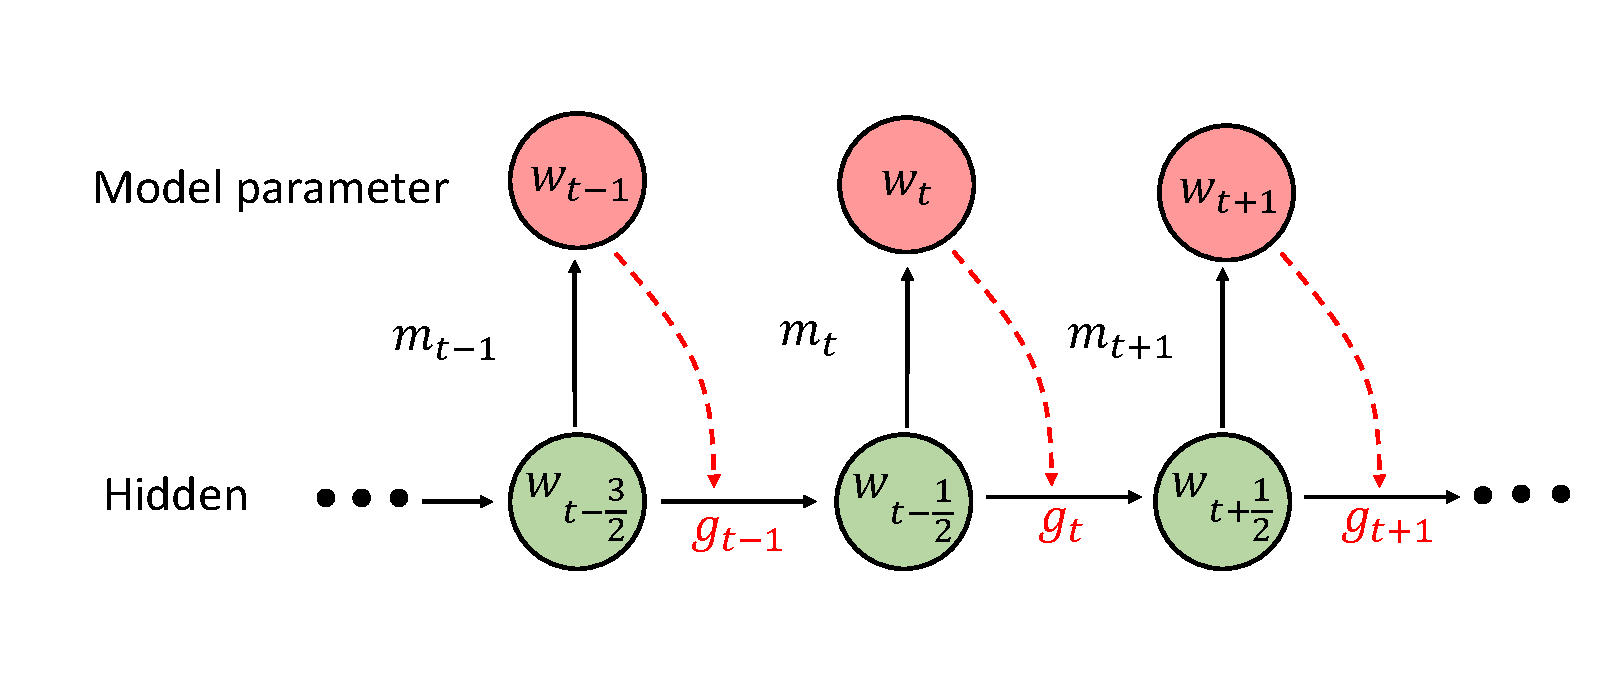
\includegraphics[width=2.6in]{plot.pdf}
    \caption{Scheme of \textsc{OPTIMISTIC-AMSGRAD}.}
     \label{scheme}
\end{figure}

\end{minipage}
\end{tabular}


We see that the proposed \textsc{Optimistic-AMSGrad} inherits three properties:
%\vspace{-0.1in}
\begin{itemize}
\item Adaptive learning rate of each dimension as \textsc{AdaGrad} \cite{DHS11}. (line 6, line 8 and line 9)
\item Exponential moving average of the past gradients as \textsc{Nesterov's method} \cite{N04} and the \textsc{Heavy-Ball} method \cite{P64}. (line 5)
\item Optimistic update that exploits a good guess of the next gradient vector
as optimistic online learning algorithms \cite{CJ12,RS13,SALS15}. (line 9)
\end{itemize}
%\vspace{-0.1in}

The first property helps for acceleration when the gradient has a sparse structure.
The second one is from the well-recognized idea of momentum which can also help for acceleration. The last one, perhaps less known outside the \textsc{Online learning} community, can actually lead to acceleration when the prediction of the next gradient is good. This property will be elaborated in the following subsection in which we provide the theoretical analysis of \textsc{Optimistic-AMSGrad}.


Observe that the proposed algorithm does not reduce to \textsc{AMSGrad} when $m_{t}=0$.
Furthermore, if $\K = \mathbb R^{d}$ (unconstrained case),
one might want to combine line 8 and line 9 and get a single line as $w_{t+1}=
w_{t-\frac{1}{2}} - \eta_t \frac{\theta_t}{ \sqrt{\hat{v}}_t } - \eta_{t+1} \frac{h_{t+1}}{ \sqrt{\hat{v}}_t }$. Yet,
based on this expression, we see that
$w_{t+1}$ is updated from $w_{t-\frac{1}{2}}$
instead of $w_t$. Therefore, while \textsc{Optimistic-AMSGrad} looks like just doing an additional update compared to \textsc{AMSGrad}, the difference of the updates is subtle.
In the following analysis, we show that the interleaving actually leads to some cancellation in the regret bound.

%\vspace{-0.15in}


\subsection{Theoretical analysis}
In this section, we provide regret analysis of the proposed method and show that it may improve the bound of vanilla \textsc{AMSGrad} with good guess of gradient.

\textbf{Notations.}\hspace{0.1in}To begin with, let us introduce some notations first.
We denote the Mahalanobis norm $\|\cdot\|_H := \sqrt{ \langle \cdot, H \cdot \rangle }$ for some PSD matrix $H$.
We let $\psi_t(x) := \langle x, \text{diag}\{\hat{v}_t\}^{1/2} x \rangle$ for a PSD matrix $H_t^{1/2}:= \text{diag}\{\hat{v}_t\}^{1/2}$, 
%Denote the PSD matrix $H_t := \text{diag}\{\hat{v}_t\}$, 
where $\text{diag}\{\hat{v}_t\}$ represents the diagonal matrix whose $i_{th}$ diagonal element is $\hat{v}_t[i]$ in Algorithm~\ref{optadam}.
We define its corresponding Mahalanobis norm $\| \cdot \|_{\psi_t}:= 
\sqrt{ \langle \cdot, \text{diag}\{\hat{v}_t\}^{1/2} \cdot \rangle }$,
where we abuse the notation $\psi_t$ to represent the PSD matrix $H_t^{1/2}:=\text{diag}\{\hat{v}_t\}^{1/2}$.
Consequently,
$\psi_t(\cdot)$ is 1-strongly convex with respect to the norm $\| \cdot \|_{\psi_t}:= 
\sqrt{ \langle \cdot, \text{diag}\{\hat{v}_t\}^{1/2} \cdot \rangle }$.
Namely, $\psi_t(\cdot)$ satisfies
$\psi_t(u) \geq \psi_t(v) + \langle \psi_t(v), u - v \rangle + \frac{1}{2} \| u - v\|^2_{\psi_t}$
for any point $u,v$.
A consequence of 1-strongly convexity of $\psi_t(\cdot)$ is that
$B_{\psi_t}(u,v) \geq \frac{1}{2} \| u - v \|^2_{\psi_t}$,
where the Bregman divergence $B_{\psi_t}(u,v)$ is defined as 
$B_{\psi_t}(u,v) := \psi_t(u)
- \psi_t(v) - \langle \psi_t(v), u - v \rangle
$ with $\psi_t(\cdot)$ as the distance generating function.
We can also define the corresponding dual norm $\| \cdot \|_{\psi_t^*}:= \sqrt{ \langle \cdot, \text{diag}\{\hat{v}_t\}^{-1/2} \cdot \rangle }$.

\textbf{Regret analysis.}\hspace{0.1in}We prove the following result regarding the regret in the convex optimization setting. That is, we assume that the loss function $f$ is convex. We also assume that $\K$ has bounded diameter $D_{\infty}$, which is a standard assumption in previous works \cite{RKK18,KB15} on adaptive methods. It is necessary in regret analysis since if the boundedness assumption is lifted, one might construct a scenario such that the benchmark is $w^* = \infty$ and the learner's regret is infinite. For simplicity, we analyze the case when $\beta_{1}=0$. One might extend our analysis to more general settings. For conciseness, we place all the proofs in the supplementary material.

\begin{Theorem} \label{thm:main}
Let $\beta_{1}=0$. Suppose the learner incurs a sequence of convex loss functions $\{ \ell_{t}(\cdot) \}$.
\textsc{Optimistic-AMSGrad} (Algorithm~\ref{optadam}) 
has regret 
\begin{equation} \label{bound:optada}
\begin{aligned}
\textstyle
 \text{Regret}_T & \textstyle
 \leq
  \frac{1}{\eta_{\min}} D_{\infty}^2 
\sum_{i=1}^d \hat{v}_{T}^{1/2}[i]
+ \frac{ B_{\psi_1}(w^*, w_{1/2})}{\eta_1} \\
&\hspace{1in}+
 \sum_{t=1}^T
\frac{\eta_t}{2} \| g_t - m_t  \|_{\psi_{t-1}^*}^2 ,
\end{aligned}
\end{equation}
where $g_{t}:= \nabla \ell_{t}(w_t)$ and $\eta_{{\min}} := \min_{{t}} \eta_{t}$.
The result holds for any benchmark $w^{*} \in \K$ and any step size sequence $\{ \eta_t \}$.
\end{Theorem}
We have the following corollary with further assumptions on $v_t$.
\begin{Corollary}
Suppose that $v_{t}$ is always monotone increasing (i.e. $\hat{v}_t = v_t, \forall t$).
Then, 
% $\text{Regret}_T \leq $
%\vspace{-0.05in}
\begin{equation} \label{bc}
\begin{aligned}
\textstyle & \textstyle \text{Regret}_T \leq 
  \textstyle
 \frac{ B_{\psi_1}(w^*, w_{1/2}) 
}{\eta_1} 
+
\sum_{t=1}^T
\frac{\eta_t}{2} \|g_t - m_t  \|_{\psi_{t-1}^*}^2 \\
&+\frac{D_{\infty}^2}{\eta_{\min}} \sum_{i=1}^d \{ (1-\beta_2) \sum_{s=1}^{T} \beta_2^{T-s} (g_s[i] - m_s[i])^2 \}^{1/2}.
\end{aligned}
\end{equation}
\end{Corollary}

We should compare the bound of (\ref{bc}) \footnote{The following conclusion in general holds for (\ref{bound:optada}), when $v_t$ may not be monotone-increasing. For brevity, we only consider the case that $\hat{v}_t=v_t$, as $\hat{v}_T$ has a clean expression in this case.}
 with that of \textsc{AMSGrad} \cite{RKK18},
which is 
\textit{
\begin{equation} \label{boundAMS}
\begin{aligned}
\textstyle
& \textstyle
 \text{Regret}_T \leq
\textstyle
 \frac{ \eta \sqrt{ 1 + \log T}    }{ (1-\beta_1)^2(1 - \gamma) \sqrt{1 - \beta_2}  } \sum_{i=1}^d \| g_{1:T}[i]  \|_2\\
 &+\frac{\sqrt{T}}{2 \eta (1 - \beta_{1})}
D^2_{\infty} \sum_{i=1}^d \hat{v}_T[i]^2 
%\\& \textstyle
 + 
D^2_{\infty} \sum_{t=1}^T \sum_{i=1}^d
\frac{\beta_{1} \hat{v}_t[i]^{1/2} }{2 \eta_t (1-\beta_1)},
\end{aligned}
\end{equation}
}
where the result was obtained by setting the step size $\eta_t = \eta /\sqrt{t}$. 
Notice that $\hat{v}_t$ in (\ref{boundAMS}) is the one in Algorithm~\ref{amsgrad} (\textsc{AMSGrad}).
For fair comparison, let us set $\eta_t=\eta/\sqrt{t}$ in (\ref{bc}) so that $\eta_1=\eta$ and $\eta_{min}= \eta/ \sqrt{T}$ and also let us set $\beta_{1}=0$ in (\ref{boundAMS}) so that their parameters have the same values.
By comparing the last term in (\ref{bc}) and the second term in (\ref{boundAMS}),
we clearly see that if $g_{t}$ and $m_{t}$ are close, the first term in (\ref{bc}) would be 
smaller than $\frac{\sqrt{T}}{2 \eta (1 - \beta_{1})} D^2_{\infty} \sum_{i=1}^d \hat{v}_T[i]^2$
of (\ref{boundAMS}).
Now let us switch to the first term in (\ref{bc}) and last term in (\ref{boundAMS}). We
see that $\frac{ B_{\psi_1}(w^*, w_{1/2}) 
}{\eta_1} \simeq D_{\infty}$ in (\ref{bc}), while $0$ in (\ref{boundAMS}).
For the second term in (\ref{bc}), we have
\begin{align*}
    &\textstyle \sum_{t=1}^T \frac{\eta_t}{2} \|g_t - m_t  \|_{\psi_{t-1}^*}^2\\
    &=\sum_{t=1}^{T-1} \frac{\eta_t}{2} \|g_t - m_t  \|_{\psi_{t-1}^*}^2
    + \eta_T \sum_{i=1}^d \frac{ (g_{T}[i] - m_{T}[i])^2 }{ \sqrt{ v_{T-1}[i]} }\\
    &=\sum_{t=1}^{T-1} \frac{\eta_t}{2} \|g_t - m_t  \|_{\psi_{t-1}^*}^2
    \\
    &\hspace{0.3in}+ \eta \sum_{i=1}^d \frac{ (g_{T}[i] - m_{T}[i])^2 }{ \sqrt{ T \big( (1-\beta_2) \sum_{s=1}^{T-1} \beta_2^{T-1-s} (g_{s}[i] - m_{s}[i])^2 } \big) }\\
    &\leq 
    \eta \sum_{i=1}^d \sum_{t=1}^T \frac{ (g_{t}[i] - m_{t}[i])^2 }{ \sqrt{ t \big( (1-\beta_2) \sum_{s=1}^{t-1} \beta_2^{t-1-s} (g_{s}[i] - m_{s}[i])^2 } \big) }.
\end{align*}
To interpret the bound, let us make a rough approximation such that
$\sum_{s=1}^{t-1} \beta_2^{t-1-s} (g_{s}[i] - m_{s}[i])^2  \simeq (g_{t}[i] - m_t[i])^2 $.
Then, we can further get an upper-bound as \begin{align*}
    \sum_{t=1}^T \frac{\eta_t}{2} \|g_t - m_t  \|_{\psi_{t-1}^*}^2 &\leq
    \frac{\eta}{\sqrt{1 - \beta}} \sum_{i=1}^d \sum_{t=1}^{T} \frac{ | g_{t}[i] - m_{t}[i] | }{ \sqrt{t} }\\
    &\leq \frac{\eta \sqrt{1 + \log T}}{\sqrt{1 - \beta}} \sum_{i=1}^d \| (g-m)_{1:T}[i] \|_2 ,
\end{align*}
where the last inequality is due to Cauchy-Schwarz. So the bound means that when
$g_{t}$ and $m_t$ are sufficiently close, the last term in (\ref{bc})
is smaller than that in (\ref{boundAMS}).
To conclude, as the second term in (\ref{bc}) (which is approximately $D_{\infty}$) is likely to be dominated by the other terms, the proposed algorithm improves \textsc{AMSGrad} when the good guess $m_t$ is available.


\subsection{Comparison to some related methods} \label{app:related}

\textbf{Comparison to nonconvex optimization works.}\hspace{0.1in}Recently, \cite{ZRSKK18,CLSH19,WWB18,ZTYCG18,ZS18,LO18} provide some theoretical analysis 
of \textsc{Adam}-type algorithms when applying them to smooth nonconvex optimization problems.
For example, \cite{CLSH19} provides a bound,
which is $\min_{t \in [T]} \mathbb{E}[\| \nabla f(w_t) \|^2 ] = O(\log T / \sqrt{T}) $.
Yet, this data independent bound does not show any advantage over standard stochastic gradient descent. Similar concerns appear in other papers.

To get some adaptive data dependent bound (e.g. bounds like (\ref{bc}) or (\ref{boundAMS})
that are in terms of the gradient norms observed along the trajectory) when applying 
\textsc{Optimistic-AMSGrad} to nonconvex optimization,
one can follow the approach of \cite{Princeton18} or \cite{CYYZC19}.
They provide ways to convert algorithms with adaptive data dependent regret bound
for convex loss functions (e.g. \textsc{AdaGrad}) to the ones that can find an approximate stationary point of non-convex loss functions. 
Their approaches are modular so that simply using \textsc{Optimistic-AMSGrad}
as the base algorithm in their methods will immediately lead to a variant of \textsc{Optimistic-AMSGrad} that enjoys some guarantee on nonconvex optimization.
The variant can outperform the ones instantiated by other \textsc{Adam}-type algorithms when
the gradient prediction $m_t$ is close to $g_t$.
The details are omitted since this is a straightforward application.

\textbf{Comparison to AO-FTRL \cite{MY16}.}\hspace{0.1in}In \cite{MY16}, the authors propose AO-FTRL, which has the update of 
the form $w_{t+1} = \arg\min_{{w \in \K}} ( \sum_{s=1}^t g_s )^{\top}  w + m_{t+1}^\top w + r_{0:t}(w) $, where $r_{0:t}(\cdot)$ is a 1-strongly convex loss function with respect to some norm $\| \cdot\|_{(t)}$ that may be different for different iteration $t$. 
Data dependent regret bound was provided in the paper, which is $r_{{0:T}}(w^*) + \sum_{t=1}^T \| g_t - m_t \|_{(t)^*}$ for any benchmark $w^{*} \in \K$. We see that if
one selects $r_{0:t}(w) := \langle w, \text{diag}\{\hat{v}_t\}^{1/2} w \rangle$ 
and $\| \cdot \|_{(t)}:= 
\sqrt{ \langle \cdot, \text{diag}\{\hat{v}_t\}^{1/2} \cdot \rangle }$, then the update might be viewed as an optimistic variant of $\textsc{AdaGrad}$. However, no experiments was provided in \cite{MY16}. 


\textbf{Comparison to \textsc{Optimistic-Adam}~\cite{DISZ18}.}\hspace{0.1in}We are aware that \cite{DISZ18} proposed one version of optimistic algorithm for ADAM, which
is called \textsc{Optimistic-Adam} in their paper. A slightly modified version is summarized in Algorithm~\ref{OPT-DISZ}. Here, \textsc{Optimistic-Adam$+\hat{v}_t$} is \textsc{Optimistic-Adam} in \cite{DISZ18} with the additional max operation $\hat{v}_t = \max ( \hat{v}_{t-1}, v_t)$ to guarantee that the weighted second moment is monotone increasing.

\begin{algorithm}[h]
\begin{algorithmic}[1]
\caption{\textsc{Optimistic-Adam~\cite{DISZ18}+$\hat{v}_t$}. \label{OPT-DISZ}}
\STATE Required: parameter $\beta_1$, $\beta_2$, and $\eta_t$.
\STATE Init: $w_1 \in \K$ and $\hat{v}_0 = v_{0} = \epsilon 1 \in \rset^{d}$.
\FOR{$t=1$ to $T$}
\STATE Get mini-batch stochastic gradient vector $g_t \in \rset^d$ at $w_t$.
\STATE $\theta_t = \beta_{1} \theta_{t-1} + (1 - \beta_{1}) g_t$.
\STATE $v_t = \beta_2 v_{t-1} + (1 - \beta_2) g_t^2$.
\STATE $\hat{v}_t = \max( \hat{v}_{t-1} , v_t )$.
\STATE $w_{t+1} = \Pi_{k}[ w_{t} - 2 \eta_t \frac{\theta_t}{ \sqrt{\hat{v}_t }}
+ \eta_t \frac{\theta_{t-1}}{ \sqrt{\hat{v}_{t-1}} }]$.
\ENDFOR
\end{algorithmic}
\end{algorithm}

We want to emphasize that the motivations are different. \textsc{Optimistic-Adam} in their paper is designed to optimize two-player games (e.g. GANs \cite{goodfellow2014generative}),
while the proposed algorithm in this paper is designed to accelerate optimization
(e.g. solving empirical risk minimization quickly).
\cite{DISZ18} focuses on training GANs \cite{goodfellow2014generative}. GANs is a two-player zero-sum game. There have been some related works in \textsc{Optimistic Online learning} like \cite{CJ12,RS13,SALS15})
showing that if both players use some kinds of $\textsc{Optimistic}$-update,
then accelerating the convergence to the equilibrium of the game is possible.
\cite{DISZ18} was inspired by these related works and showed that \textsc{Optimistic-Mirror-Descent}
can avoid the cycle behavior in a bilinear zero-sum game, which accelerates the convergence. Furthermore, \cite{DISZ18} did not provide theoretical analysis of \textsc{Optimistic-Adam}.

%\vspace{-0.05in}
\section{Gradient Prediction} \label{sec:predict_m}

From the analysis in the previous section, we know that whether \textsc{Optimistic-AMSGrad}
converges faster than its counterpart depends on how $m_{t}$ is chosen.
In \textsc{Optimistic-Online learning}, $m_{t}$ is usually set to $m_{t}= g_{t-1}$,
which means that it uses the previous gradient as a guess of the next one.
The choice can accelerate the convergence to equilibrium in some two-player zero-sum games
\cite{RS13,SALS15,DISZ18}, in which each player uses an optimistic online learning algorithm
against its opponent.

However, this paper is about solving optimization problems instead of solving zero-sum games. 
We propose to use the extrapolation algorithm of \cite{SAB16}.
Extrapolation studies estimating the limit of sequence using the last few iterates
\cite{BZ13}. 
Some classical works include Anderson acceleration \cite{WN11}, minimal polynomial extrapolation \cite{CJ76}, reduced rank extrapolation \cite{E79}.
These methods typically assume that the sequence $\{x_t\} \in \mathbb R^d$
has a linear relation
\begin{equation} \label{vvv}
x_t = A( x_{t-1} - x^* ) + x^*,
\end{equation}
and $A \in \mathbb R^{d \times d}$ is an unknown, not necessarily symmetric, matrix.
The goal is to find the fixed point of $x^{*}$.
\cite{SAB16} relaxes the assumption to certain degrees.
It assumes that the sequence $\{x_t\} \in \mathbb R^d$ satisfies
\begin{equation} \label{nox}
x_t - x^* = A( x_{t-1} - x^* ) + e_t,
\end{equation}
where $e_t$ is a second order term satisfying $\| e_t \|_2  = O( \| x_{t-1} - x^* \|_2^2)$
and $A \in \mathbb R^{d \times d}$ is an unknown matrix.
The extrapolation algorithm we used is shown in Algorithm~\ref{algex}.
Some theoretical guarantees regarding the distance between the output and $x^*$ are provided in \cite{SAB16}.

\begin{algorithm}[h]
\begin{algorithmic}[1] 
\small
\caption{\textsc{Regularized Approximate Minimal Polynomial Extrapolation} (RMPE)
\cite{SAB16} } \label{algex}
\STATE \textbf{Input:} sequence $\{ x_s \in \mathbb R^d \}_{s=0}^{s=r}$, parameter $\lambda > 0$.
\STATE Compute matrix  $U = [ x_1 - x_0, \dots, x_{r} - x_{r-1}] \in \mathbb R^{d \times r}$.
\STATE Obtain $z$ by solving $(U^\top U + \lambda I ) z = \mathbf{1}$.
\STATE Get $c= z / (z^\top \mathbf{1})$.
\STATE \textbf{Output:} $\Sigma_{i=0}^{r-1} c_i x_i$, the approximation of the fixed point $x^*$.
\end{algorithmic}
\end{algorithm}


For \textsc{Optimistic-AMSGrad},
we use Algorithm~\ref{algex} to get $m_t$.
Specifically, $m_t$ is obtained by
\begin{itemize}
\item Call Algorithm~\ref{algex} with input being a sequence of some past $r+1$ gradients, $\{ g_t, g_{t-1},g_{t-2}, \dots, g_{t-r} \}$, %to obtain $m_t$,
where $r$ is a parameter.
\item Set $m_t:= \Sigma_{i=0}^{r-1} c_i g_{t-r+i}$ from the output of Algorithm~\ref{algex}.
\end{itemize}


To see why the output from the extrapolation method may be a reasonable estimation, assume that the update converges to
a stationary point (i.e. $g^*:=\nabla f(w^*) = 0$ for the underlying function $f$).
Then, we might rewrite (\ref{nox}) as
\begin{equation} \label{key_to_comp}
g_t = A g_{t-1}  + O( \| g_{t-1} \|_2^2 ) u_{t-1},
\end{equation}
for some vector $u_{t-1}$ with a unit norm.
The equation suggests that the next gradient vector $g_{t}$ is a linear transform of $g_{{t-1}}$
plus an error vector that may not be in the span of $A$ whose length is $O( \| g_{t-1} \|_2^2 )$.
If the algorithm is guaranteed to converge to a stationary point, the magnitude of the error component will eventually go to zero.

We remark that the choice of algorithm for gradient prediction is surely not unique. We propose to use the recent result among various related works. Indeed, one can use any method that can provide reasonable guess of gradient in next iteration.

\noindent
\textbf{Two illustrative examples.}\hspace{0.1in}We provide two toy examples to demonstrate how \textsc{OPTIMISTIC-AMSGrad} works with the chosen extrapolation method. First, consider minimizing a quadratic function $H(w) := \frac{b}{2} w^2 $  
%The eigenvalue of matrix $B \in \mathbb R^{d \times d}$ can be negative.
with vanilla gradient descent method $w_{t+1} = w_t - \eta_t \nabla H(w_t)$. 
The gradient $g_{t}:= \nabla H(w_{t})$ has a recursive description as 
$g_{t+1} = b w_{t+1} = b ( w_t  - \eta_t g_t ) = g_t - b \eta_t g_t  $.
So, the update can be written in the form of (\ref{key_to_comp}) 
with $A = (1 - b \eta)$ and $u_{t-1}=0$ by setting $\eta_t=\eta$ (constant step size).
Therefore, the extrapolation method should predict well.


%\vspace{-0.05in}
\begin{figure}[t]
\centering
    \mbox{
    \includegraphics[width=0.25\textwidth]{./simulation/fig/fig1_left.eps}
    \includegraphics[width=0.25\textwidth]{simulation/fig/fig1_right.eps}
    }
    \mbox{
    \includegraphics[width=0.25\textwidth]{./simulation/fig/fig2_left.eps}
    \includegraphics[width=0.25\textwidth]{simulation/fig/fig2_right.eps}
    }
     \caption{\small (a): The iterate $w_t$; the closer to the optimal point $0$ the better. (b): A scaled and clipped version of $m_t$: $w_t - w_{t-1/2}$, which measures how the prediction of $m_t$ drives the update towards the optimal point. In this scenario, the more negative the better.
     (c): Distance to the optimal point $-1$. The smaller the better. (d): A scaled and clipped version of $m_t$: $w_t - w_{t-1/2}$, which measures how the prediction of $m_t$ drives
the update towards the optimal point. In this scenario, the more negative the better.
     }
     \label{simu}
\vspace{-0.2in}
\end{figure}

Specifically, consider optimizing $H(w) := w^2/2 $ 
by the following three algorithms with the same step size.
One is Gradient Descent (GD): $w_{t+1} = w_t - \eta_t g_t$,
while the other two are
\textsc{Optimistic-AMSGrad} with $\beta_1=0$ and the second moment term $\hat{v}_t$ being dropped: 
$w_{t+\frac{1}{2}} = \Pi_{\K}\big[ w_{t-\frac{1}{2}} - \eta_t g_t \big]$,
$w_{t+1} = \Pi_{\K}\big[ w_{t+\frac{1}{2}} - \eta_{t+1} m_{t+1} \big]$.
We denote the algorithm that sets $m_{t+1}= g_t$ as Opt-1,
and denote the algorithm that uses the extrapolation method
to get $m_{t+1}$ as Opt-extra.
We let $\eta_t=0.1$ and the initial point $w_0=5$ for all the three methods. 
The simulation results are on Figure~\ref{simu} (a) and (b). Sub-figure (a) plots update $w_t$ over iteration, where the updates should go towards the optimal point $0$.
Sub-figure (b) is about a scaled and clipped version of $m_t$, defined as $w_t - w_{t-1/2}$,
which can be viewed as $- \eta_t m_{t}$ if the projection (if exists) is lifted.
Sub-figure (a) shows that Opt-extra converges faster than the other methods. 
Furthermore, sub-figure (b) shows that the prediction by the extrapolation
method is better than the prediction by simply using the previous gradient. The sub-figure shows that
$-m_t$ from both methods all point to $0$ in all iterations and the magnitude is larger for the one produced by the extrapolation method after iteration $2$. \footnote{
The extrapolation method needs at least two gradients for prediction.
This is why in the first two iterations, $m_t$ is $0$.
}


Now let us consider another problem: an online learning problem proposed in \cite{RKK18}
\footnote{\cite{RKK18} uses this example to show that \textsc{Adam} \cite{KB15} fails to converge.}.
Assume the learner's decision space is $\K=[-1,1]$, and
the loss function is $\ell_t(w) = 3 w$ if $t \text{ mod } 3 = 1$,
and $\ell_t(w) = - w$ otherwise.
The optimal point to minimize the cumulative loss is $w^*=-1$.
We let $\eta_t=0.1 / \sqrt{t}$ and the initial point $w_0=1$ for all the three methods.
The parameter $\lambda$ of the extrapolation method is set to $\lambda=10^{-3}>0$.
The results are on Figure~\ref{simu} (c) and (d).
Sub-figure (c) shows that Opt-extra converges faster than the other methods
while Opt-1 is not better than GD.
The reason is that the gradient changes from $-1$ to $3$ at $t \text{ mod } 3 = 1$
and it changes from $3$ to $-1$ at $t \text{ mod } 3 = 2$.
Consequently, using the current gradient as the guess for the next clearly is not a good choice,
since the next gradient is in the opposite direction of the current one.
Sub-figure (d) shows that $-m_t$ by the extrapolation method always points to
$w^*=-1$, while the one by using the previous negative direction points to the opposite direction in two thirds of rounds. It shows that the extrapolation method is much less affected by the gradient oscillation and always makes the prediction in the right direction, which suggests that the method can capture the aggregate effect.


\section{Experiments}

In this section, we provide experiments on classification tasks with various neural network architectures and datasets to demonstrate the effectiveness of \textsc{OPTIMISTIC-AMSGrad} in practical applications.

\textbf{Methods.}\hspace{0.1in}We consider two baselines. The first one is the original \textsc{AMSGrad}. 
The hyper-parameters are set to be $\beta_1$ and $\beta_2$ to be $0.9$ and $0.999$ respectively, as recommended by \cite{RKK18}. We tune the learning rate $\eta$ over a fine grid and report the best result. 

The other competing method is the aforementioned
\textsc{Optimistic-Adam$+\hat{v}_t$} method (Algorithm \ref{OPT-DISZ}) as in Section 3. The key difference is that it uses previous gradient as the gradient prediction of the next iteration. We also report the best result achieved by tuning the step size $\eta$ for \textsc{Optimistic-Adam$+\hat{v}_t$}.

\begin{figure}[t]
\vspace{-0.02in}
\begin{center}
\mbox{
\includegraphics[width=1.65in]{simulation/fig2/M_rand_train_loss_no1.eps}\hspace{-0.1in}
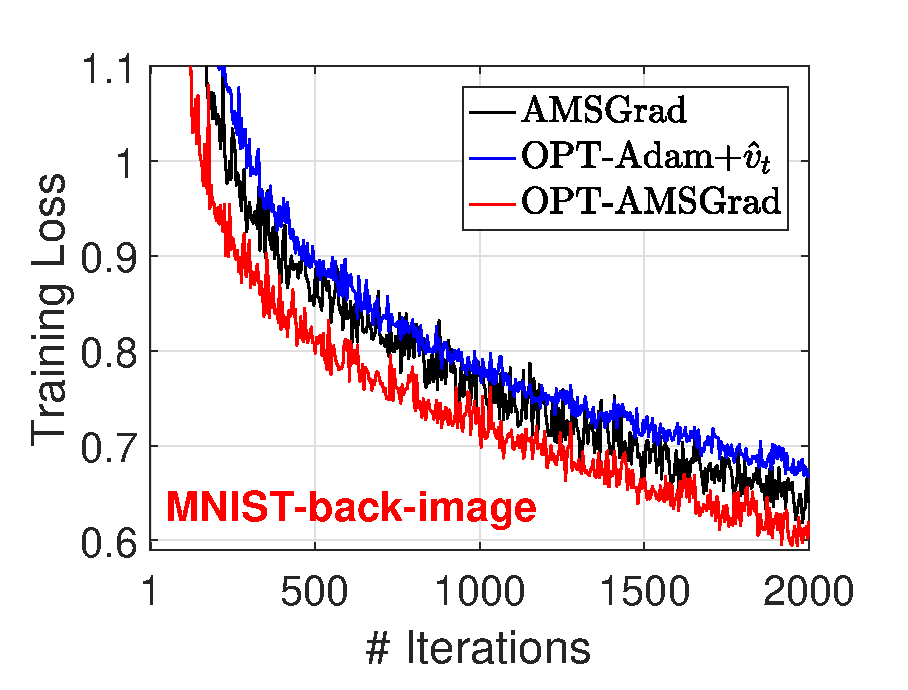
\includegraphics[width=1.65in]{simulation/fig2/M_image_train_loss_no1.eps}\hspace{-0.1in}
}
\mbox{
\includegraphics[width=1.65in]{simulation/fig2/cifar_cnn_train_loss_no1.eps}\hspace{-0.1in}
\includegraphics[width=1.65in]{simulation/fig2/imdb_lstm_train_loss_no1.eps}
}    

\mbox{
\includegraphics[width=1.65in]{simulation/fig2/cifar10_resnet_train_loss.eps}\hspace{-0.1in}
\includegraphics[width=1.65in]{simulation/fig2/cifar100_resnet_train_loss.eps}
}
\vspace{-0.02in}
\caption{Training loss vs. Number of iterations. The first row are results with fully-connected neural network.}
\label{train_loss}
\end{center}
\vspace{-0.04in}
\end{figure}

% \begin{figure}[t]
% \begin{center}
% \mbox{
% \includegraphics[width=1.65in]{simulation/fig2/M_image_train_loss_epoch.eps}\hspace{-0.1in}
% \includegraphics[width=1.65in]{simulation/fig2/cifar_cnn_train_loss_epoch.eps}\hspace{-0.1in}
% }
% \mbox{
% \includegraphics[width=1.65in]{simulation/fig2/imdb_lstm_train_loss_epoch.eps}
% \includegraphics[width=1.65in]{simulation/fig2/CIFAR100_resnet_train_loss_epoch.eps}
% }
% \end{center}
% \vspace{-0.1in}
% \caption{Training loss for the first 4 epochs. An epoch means all training samples are used once.}
% \label{Epoch}
% \vspace{-0.04in}
% \end{figure}

\begin{figure}[h]
\begin{center}
\mbox{
\includegraphics[width=1.65in]{./new_figure/new_mnist_img_figure/mnist_img_train_loss_disz_2.eps}\hspace{-0.1in}
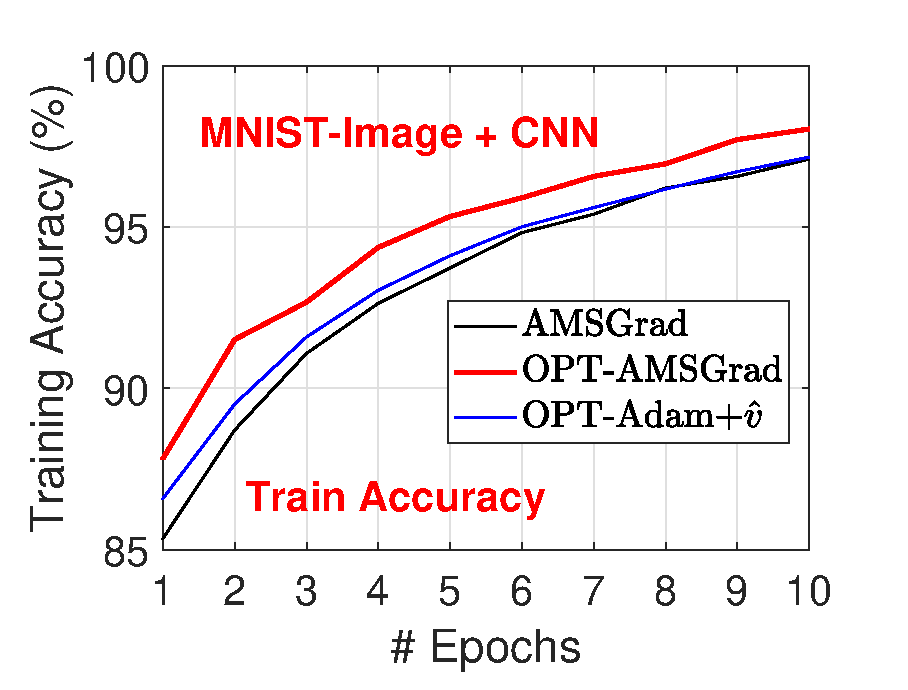
\includegraphics[width=1.65in]{./new_figure/new_mnist_img_figure/mnist_img_train_acc_disz_2.eps}
}
\mbox{
\includegraphics[width=1.65in]{./new_figure/mnist_img_test_loss_disz.eps}\hspace{-0.1in}
\includegraphics[width=1.65in]{./new_figure/mnist_img_test_acc_disz.eps}
}
\end{center}
 \caption{\textit{MNIST-back-image} + convolutional neural network.} \label{figs:M_image_new3}
\end{figure}

\begin{figure}[h]
\begin{center}
\mbox{
\includegraphics[width=1.65in]{./new_figure/cifar10_train_loss_disz.eps}\hspace{-0.1in}
\includegraphics[width=1.65in]{./new_figure/cifar10_train_acc_disz.eps}
}
\mbox{
\includegraphics[width=1.65in]{./new_figure/cifar10_test_loss_disz.eps}\hspace{-0.1in}
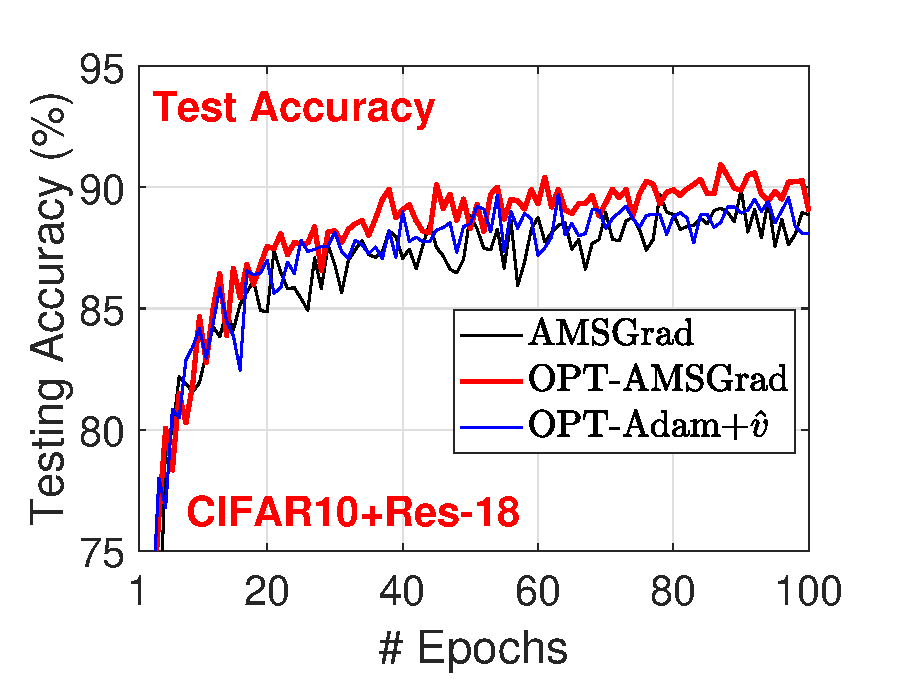
\includegraphics[width=1.65in]{./new_figure/cifar10_test_acc_disz.eps}
}
\end{center}
\caption{\textit{CIFAR10} + Res-18. We compare three methods in terms of training (cross-entropy) loss, training accuracy, testing loss, and testing accuracy. We observe that \textsc{Optimistic-AMSGrad} consistently improves the two baselines.} \label{figs:CIFAR10_new3}
\end{figure}

\begin{figure}[h]
\begin{center}
\mbox{
\includegraphics[width=1.65in]{new_figure/cifar100_train_loss_disz.eps}\hspace{-0.1in}
\includegraphics[width=1.65in]{new_figure/cifar100_train_acc_disz.eps}
}
\mbox{
\includegraphics[width=1.65in]{new_figure/cifar100_test_loss_disz.eps}\hspace{-0.1in}
\includegraphics[width=1.65in]{new_figure/cifar100_test_acc_disz.eps}
}
\end{center}
\caption{\textit{CIFAR100} + Res-50. We compare three methods in terms of training (cross-entropy) loss, training accuracy, testing loss, and testing accuracy.} \label{figs:CIFAR100_new3}
\end{figure}

For \textsc{Optimistic-AMSGrad}, we use the same $\beta_1$, $\beta_2$ and 
the best step size $\eta$ of \textsc{AMSGrad} for a fair evaluation of the improvement brought by the extra optimistic step. Yet,
\textsc{Optimistic-AMSGrad} has an additional parameter $r$ that controls the number of previous gradients used for gradient prediction. Fortunately, we observe similar performance of \textsc{Optimistic-AMSGrad} with different values of $r$. Hence, we report $r=5$ for now when comparing with other baselines. We will address on the choice of $r$ at the end of this section.

In all experiments, all the optimization algorithms are initialized at the same point. We report the results averaged over 5 repetitions.

\textbf{Datasets.}\hspace{0.1in}Following \cite{RKK18} and \cite{KB15}, we compare different algorithms on \textit{MNIST}, \textit{CIFAR10},
\textit{CIFAR100}, and \textit{IMDB} datasets. 
For \textit{MNIST}, we use two noisy variants named as 1.65\textit{MNIST-back-rand} and 1.65\textit{MNIST-back-image} from \cite{MNIST07}. They both have 12000 training samples and 50000 test samples, where random background is inserted to the original \textit{MNIST} hand written 
digit images. For \textit{MNIST-back-rand}, each image is inserted with a random background, whose pixel values generated uniformly from 0 to 255, while \textit{MNIST-back-image} takes random patches from a black and white as noisy background.
The input dimension is 784 ($28\times 28$) and the number of classes is $10$. \textit{CIFAR10} and \textit{CIFAR100} are popular computer-vision datasets consisting of 50000 training images and 10000 test images, of size $32\times 32$. The number of classes are 10 and 100, respectively. The \textit{IMDB} movie review dataset is a binary classification dataset with 25000 training and testing samples respectively. It is a popular datasets for text classification.

\textbf{Network architecture.}\hspace{0.1in}We adopt a multi-layer fully-connected neural network with input layer followed by a hidden layer with $200$ nodes, which is connected to another layer with $100$ nodes before the output layer. The activation function is ReLU for hidden layers, and softmax for the output layer. This network is tested on \textit{MNIST} variants. Since convolutional networks are popular for image classification tasks, we consider an ALL-CNN architecture proposed by \cite{CNN15}, which is constructed with several convolutional blocks and dropout layers. In addition, we also apply residual networks, Resnet-18 and Resnet-50~\cite{Rnet16}, which have achieved many state-of-the-art results. For the texture \textit{IMDB} dataset, we consider training a Long-Short Term Memory (LSTM) network. The network includes a word embedding layer with 5000 input entries representing most frequent words in the dataset, and each word is embedded into a 32 dimensional space. The output of the embedding layer is passed to 100 LSTM units, which is then connected to 100 fully connected ReLu's before the output layer. For all the models, we use cross-entropy loss. A mini-batch size of $128$ is used to compute the stochastic gradients.

\textbf{Results.}\hspace{0.1in}Firstly, to illustrate the acceleration effect of \textsc{OPTIMISTIC-AMSGrad} at early stage, we provide the training loss against number of iterations in Figure~\ref{train_loss}. We clearly observe that on all datasets, the proposed \textsc{Optimistic-AMSGrad} converges faster than the other competing methods, right after the training begins. In other words, we need fewer iterations (samples) to achieve the same training loss. This validates one of the main advantages of \textsc{Optimistic-AMSGrad}, which is a higher sample efficiency.

We are also curious about the long-term performance and generalization of the proposed method in test phase. In Figure~\ref{figs:M_image_new3}, Figure~\ref{figs:CIFAR10_new3} and Figure~\ref{figs:CIFAR100_new3}, we plot the corresponding results when the model is trained to the state with stable test accuracy. We observe: 1) In the long term, \textsc{OPTIMISTIC-AMSGrad} algorithm may converge to a better point with smaller objective function value, and 2) In this three applications, the proposed \textsc{OPTIMISTIC-AMSGrad} also outperforms the competing methods in terms of test accuracy. These are also important benefits of \textsc{OPTIMISTIC-AMSGrad}.


\subsection{Choice of parameter $r$}
Recall that our proposed algorithm has the parameter $r$ that governs the use of past information.
Figure~\ref{fig:compare-r} compares the performance under different values of $r=3,5,10$ on two datasets. From the result we see that the choice of $r$ does not have significant impact on learning performance. Taking into consideration both quality of gradient prediction and computational cost, it appears that $r=5$ is a good choice. We remark that empirically, the performance comparison among $r=3,5,10$ is not absolutely consistent (i.e. more means better) in all cases. One possible reason is that for deep neural nets which have very complicated and highly non-convex landscape, using gradient information from too long ago may not be helpful in accurate gradient prediction. Nevertheless, $r=5$ seems to be good for most applications.

\begin{figure}[]
\begin{center}
\mbox{
\includegraphics[width=1.65in]{./new_figure/new_mnist_img_figure/mnist_img_train_loss_r3510_2.eps}\hspace{-0.1in}
\includegraphics[width=1.65in]{./new_figure/cifar10_train_loss_r3510.eps}
}
\end{center}
\vspace{-0.1in}
\caption{The training loss of \textsc{OPTIMISTIC-AMSGrad} with different $r$.}     \label{fig:compare-r}
\end{figure}


\section{Concluding Remarks}
\subsection{Discussion on the iteration cost}

We observe that the iteration cost (i.e., actual running time per iteration) of our implementation of \textsc{Optimistic-AMSGrad} with $r=5$ is roughly two times larger than the standard \textsc{AMSGrad}. When $r=3$, the cost is roughly 0.7 times longer. Nevertheless, \textsc{OPTIMISTIC-AMSGrad} may still be beneficial in terms of training efficiency, since fewer iterations are typically needed. For example, in Figure \ref{figs:CIFAR10_new3} and \ref{figs:CIFAR100_new3}, to reach the training loss of \textsc{AMSGrad} at 100 epochs, the proposed method only needs roughly 20 and 40 epochs, respectively. That said, \textsc{OPTIMISTIC-AMSGrad} needs 40\% and 80\% time to achieve same training loss as \textsc{AMSGrad}, in this two problems.

The computational overhead mostly comes from the gradient extrapolation step. More specifically, recall that the extrapolation step consists of:
(a) The step of constructing the linear system $(U^\top U)$.
The cost of this step can be optimized and reduced to $\mathcal O(d)$, since the matrix $U$ only changes one column at a time.
(b) The step of solving the linear system.
The cost of this step is $O(r^3)$, which is negligible as the linear system is very small ($5$-by-$5$ if $r=5$).
(c) The step that outputs an estimated gradient as a weighted average of previous gradients.
The cost of this step is $\mathcal O(r \times d)$. Thus, the computational overhead is $\mathcal O\left((r+1)d+r^3\right)$.
Yet, we notice that step (a) and (c) is parallelizable, so they can be accelerated in practice.

\noindent \textbf{Memory usage:} Our algorithm needs a storage of past $r$ gradients for each coordinate, in addition to the estimated second moments and the moving average. Though it seems demanding compared to the standard AMSGrad, it is relatively cheap compared to Natural gradient method (e.g.,~\cite{MG15}), as Natural gradient method needs to store some matrix inverse.

\subsection{Conclusion}
In this paper, we propose \textsc{Optimistic-AMSGrad}, which combines optimistic learning and \textsc{AMSGrad} to improve sampling efficiency and
accelerate the process of training, in particular for deep neural networks. With a good gradient prediction, the regret can be smaller than that of standard \textsc{AMSGrad}. Experiments on various deep learning problems demonstrate the effectiveness of the proposed method in improving the training efficiency. 



\clearpage

\bibliographystyle{abbrvnat}
\bibliography{reference}

\clearpage


\appendix

\section{Proof of Theorem~\ref{thm:main}} \label{app:thm}

\begin{proof}

This completes the proof.
\end{proof}

%-----------------------------------------------------------------------------
%\vspace{0.4cm}

\end{document} 